\newpage
\section{SORA Payload Description}
\label{sec:Hardware}
With the successful completion of the first flight of SORA in 2017, the UH team decided to use the same materials with improved construction methods to build SORA 2.0.  The design was optimized this year to use all the space available on the 2018 flight as shown on figure ~\ref{fig:payload_dim}.   The outer shell is KYDEX, a composite made of PVC and acrylic. KYDEX	 was initially chosen due to its properties.  It is hydrophobic, UV resistant, and can withstand a wide range of conditions.  It has a tensile strength of \SI{6100} PSI and an impact strength of \SI{15.00} ft.-lbs./in.  The bolts used on the payload mainly were iron bolts with a weather-resistant coating.   Brackets and other wall-mounting parts were nickel plated off-the-shelf parts.  
%
\begin{figure}[H]
    \centering
    \begin{minipage}{0.45\textwidth}
        \centering
        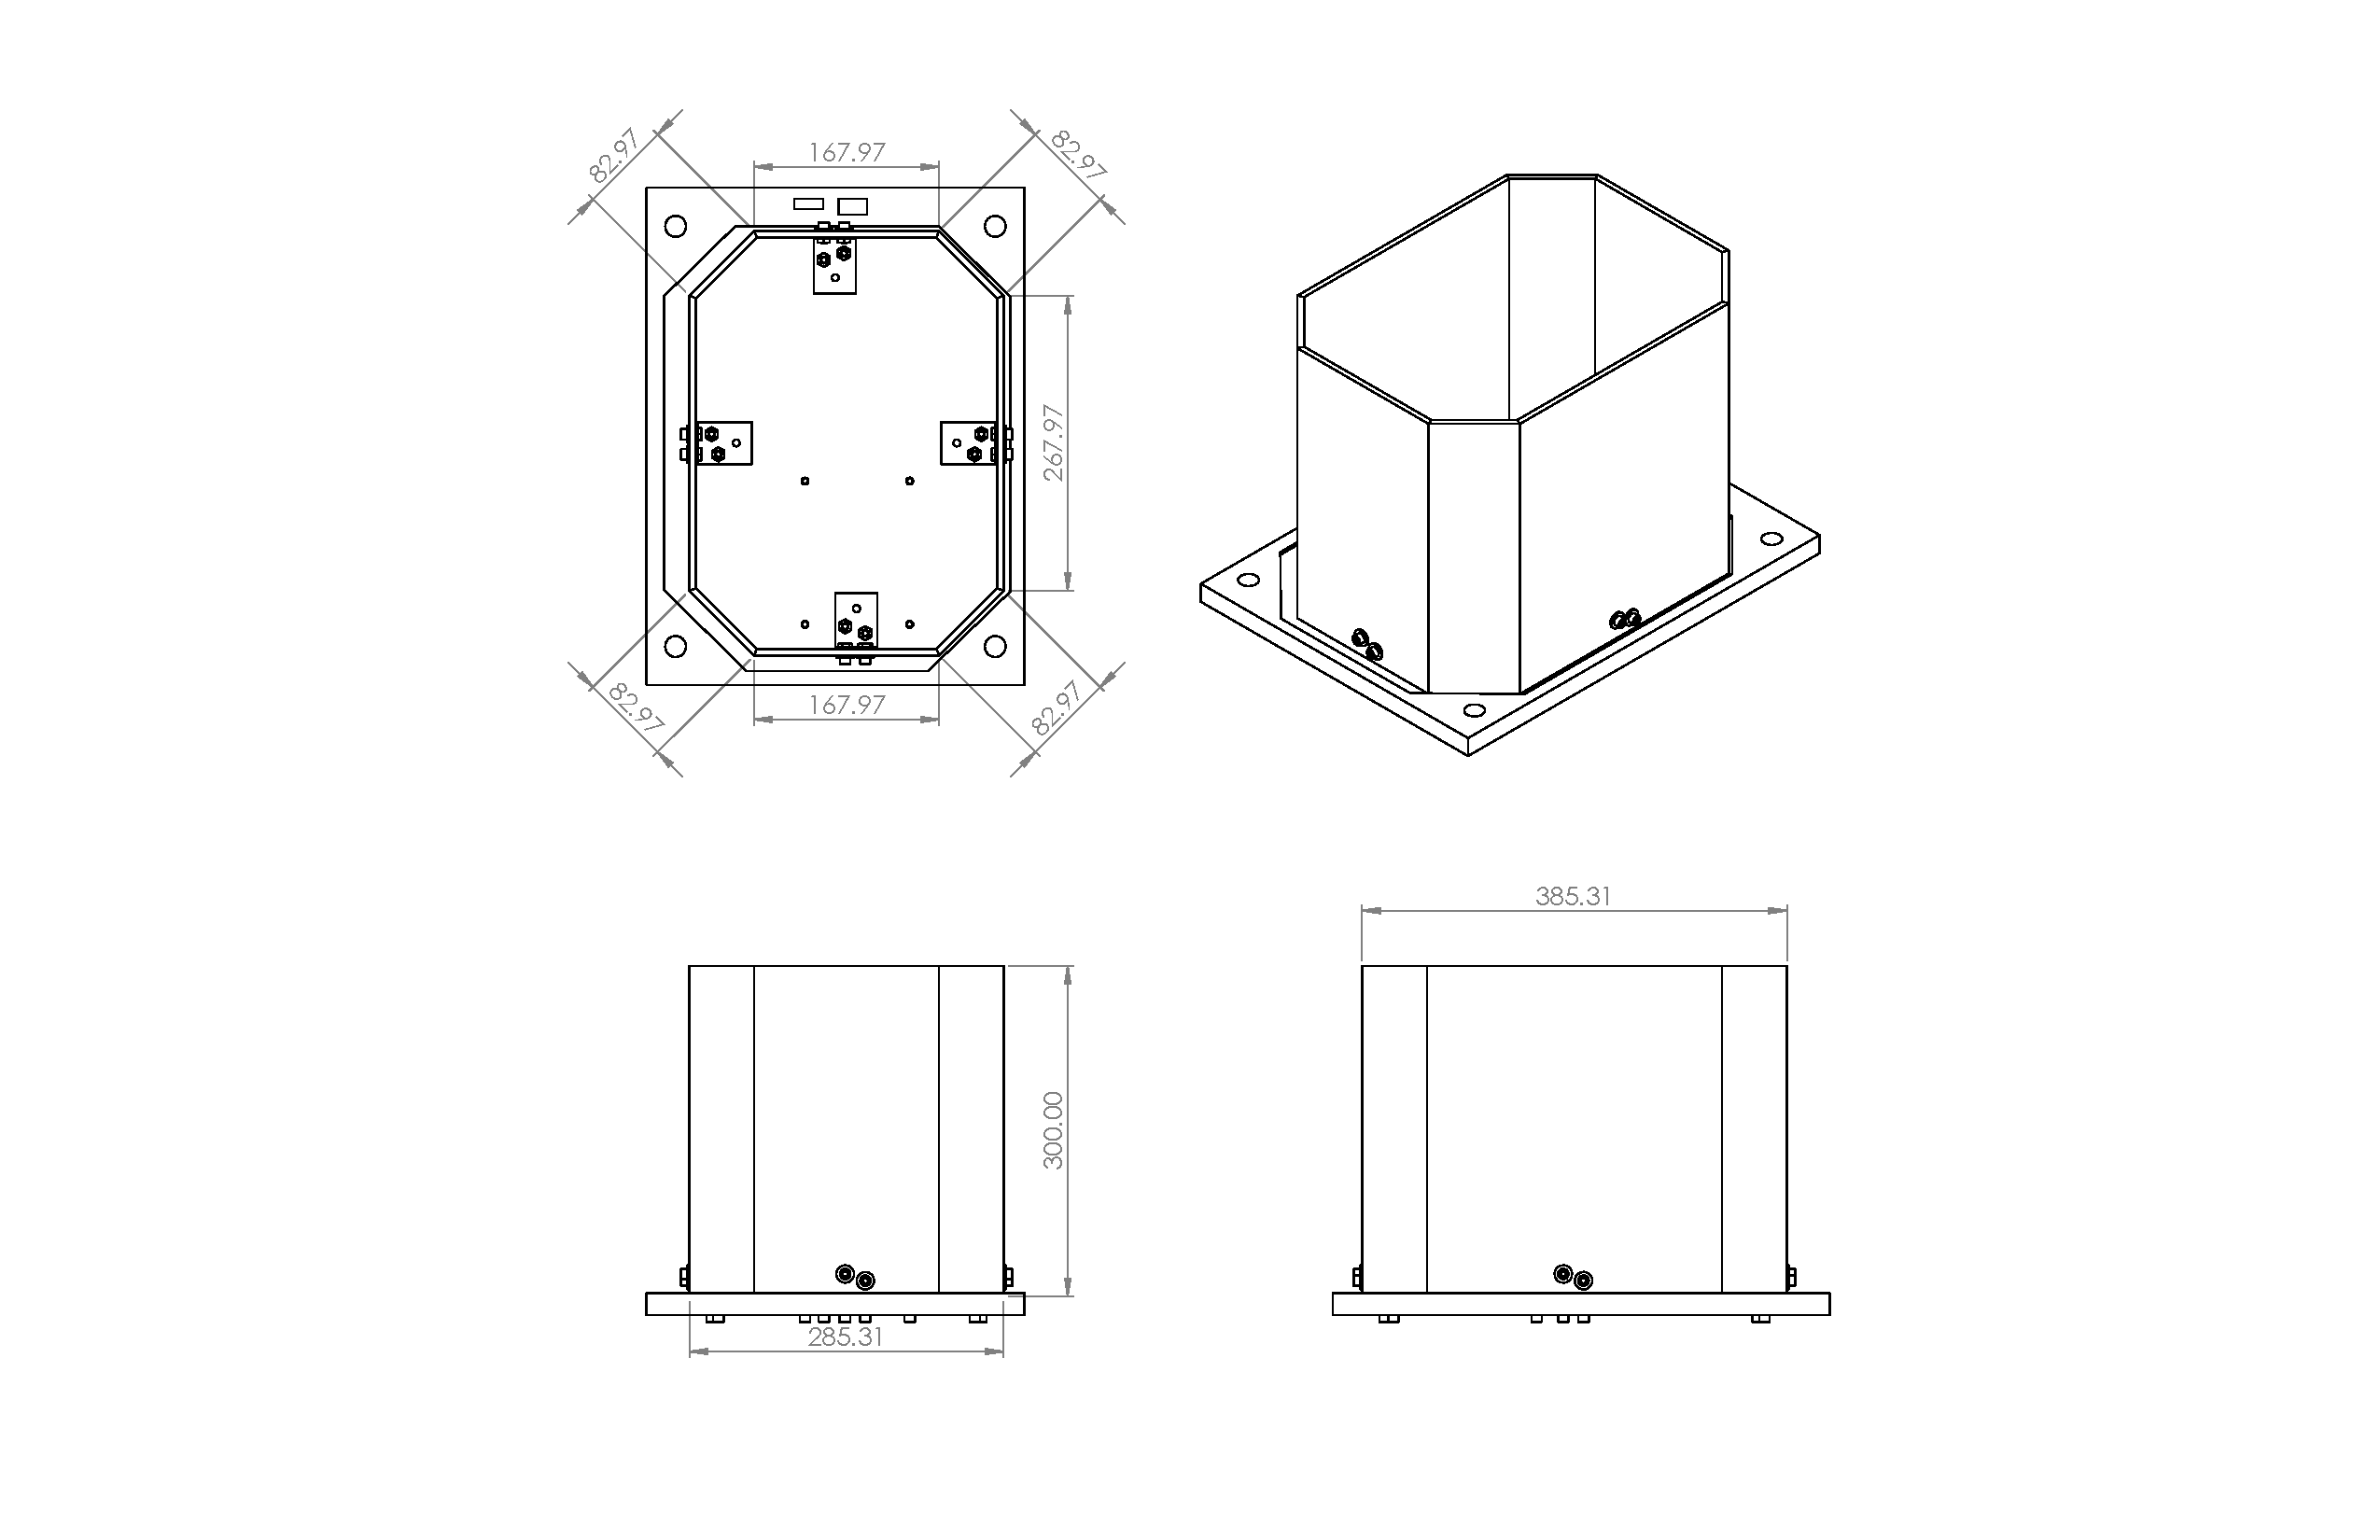
\includegraphics[width=0.9\textwidth]{figures/payload_dimensions.PDF} % first figure itself
        \caption{Payload Dimensions}
        	\label{fig:payload_dim}
    \end{minipage}\hfill
    \begin{minipage}{0.45\textwidth}
        \centering
        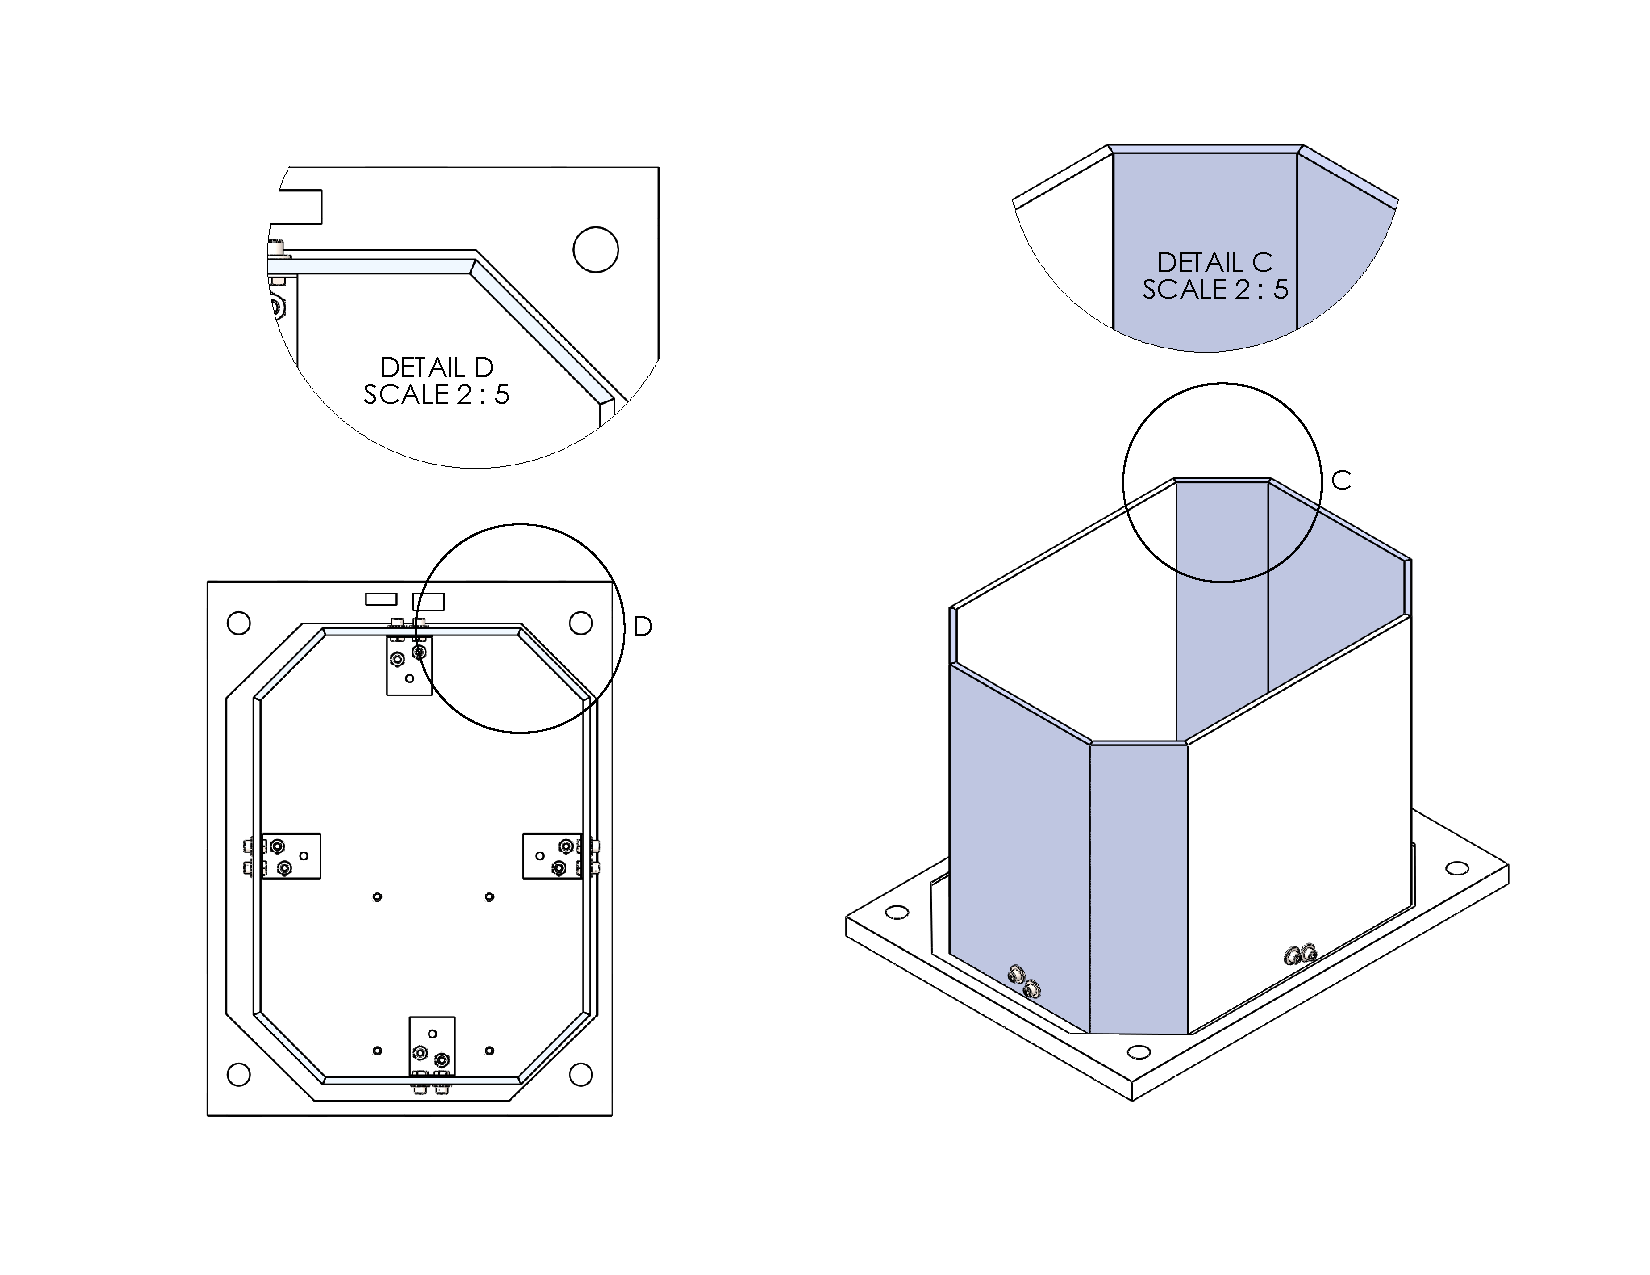
\includegraphics[width=0.9\textwidth]{figures/payload_corners.PDF} % second figure itself
        \caption{Payload Corners}
        	\label{fig:payload_corn}
    \end{minipage}
\end{figure}
%

The outer shell was machine cut to our specified dimensions, including the corners so all the walls would sit flush against each other as seen in figure ~\ref{fig:payload_corn}.  This design allowed the team to fully take advantage of every inch of space provided on the flight.  The biggest difference this year when compared to the 2017 flight is that the payload shell encompasses all the systems.  There are no external systems and this allowed the team to rearrange experiments in a more efficient manner.
The overall system organization was kept simple.  As shown in figure ~\ref{fig:payload_sec}, the payload carried a full load of scientific equipment.  The astrobiology system and the radiation MiniPIX system required specific positions as shown.  This was due to certain mechanical movements and ease of access to devices.  The rest of the electronics were positioned as close as possible to the cable access ports that HASP provided on the payload plate.

\begin{figure}[H]
    \begin{center}
        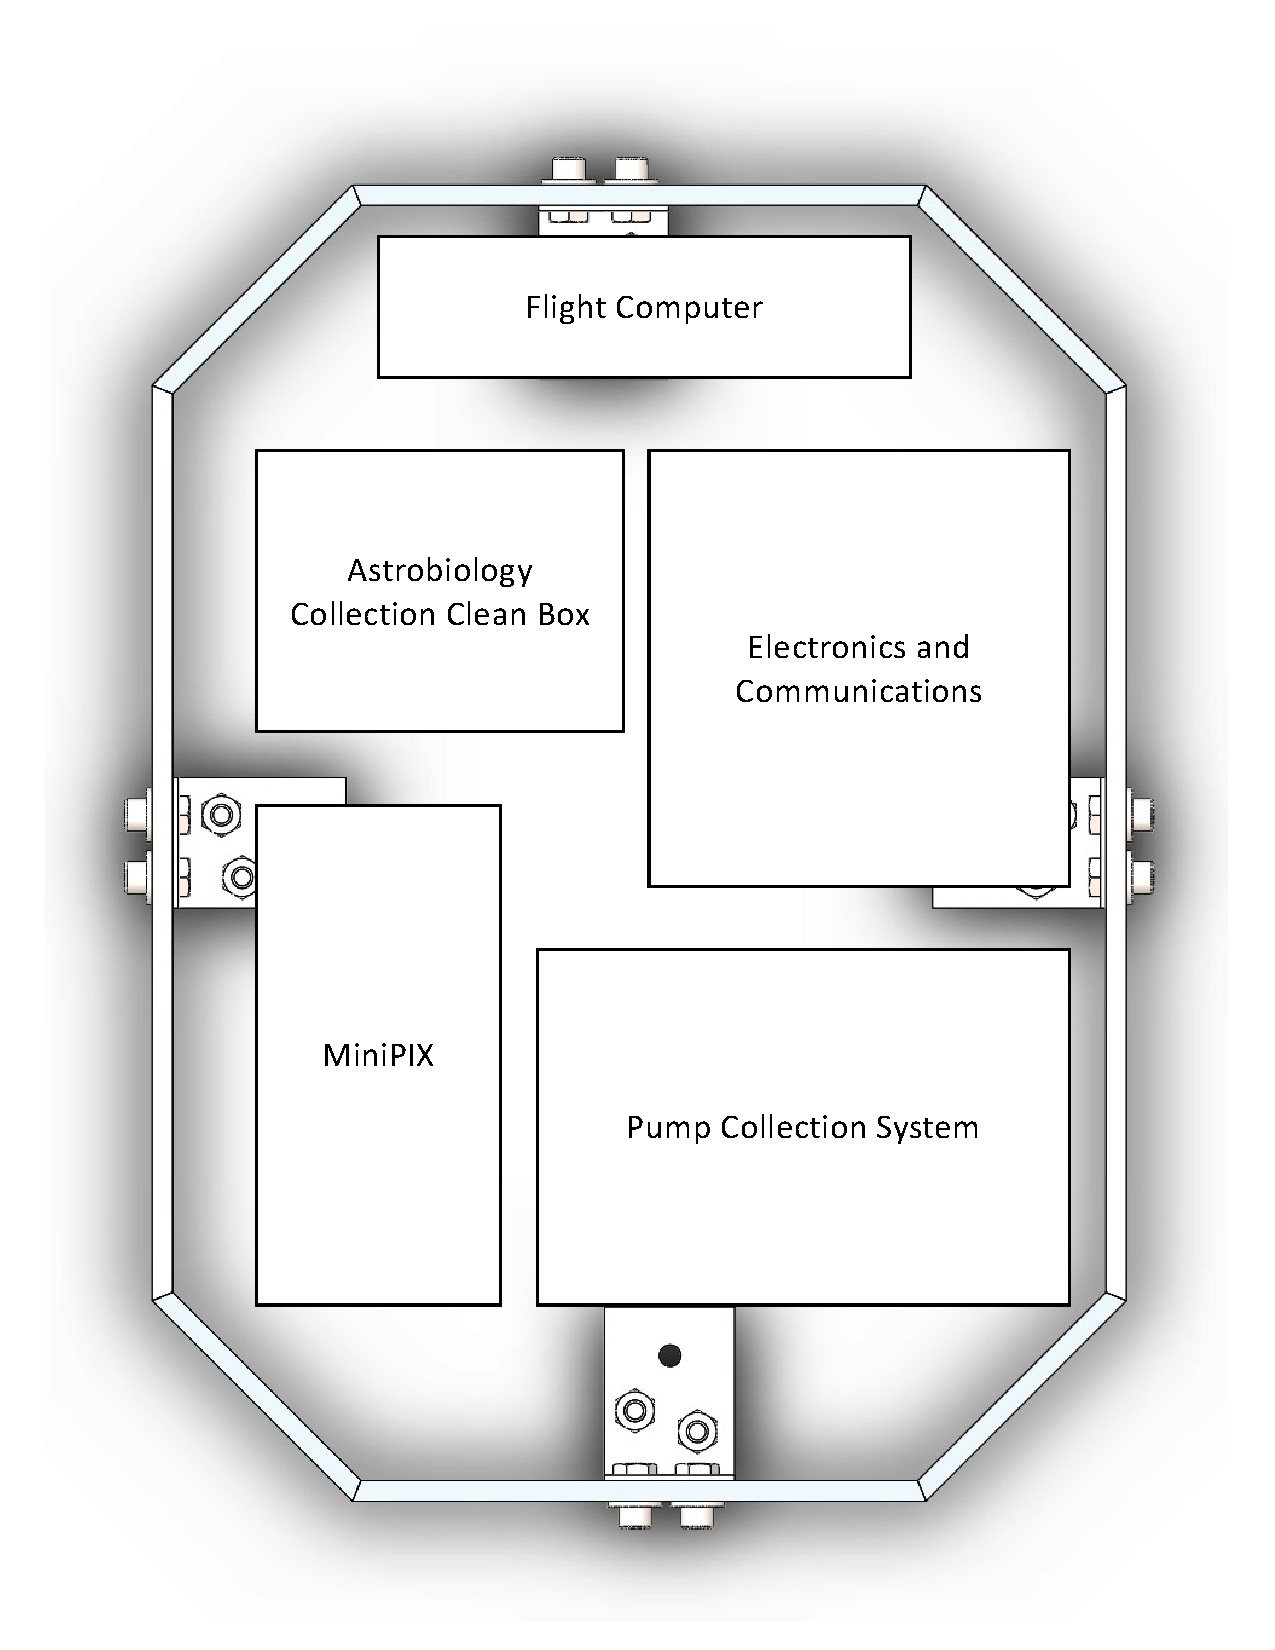
\includegraphics[width=60 mm, scale=1]{figures/payload_sections.pdf}
        \caption{Payload Sections and Space}
        \label{fig:payload_sec}
    \end{center}
\end{figure}
%\begin{figure}[t!]
%	\begin{center}
%		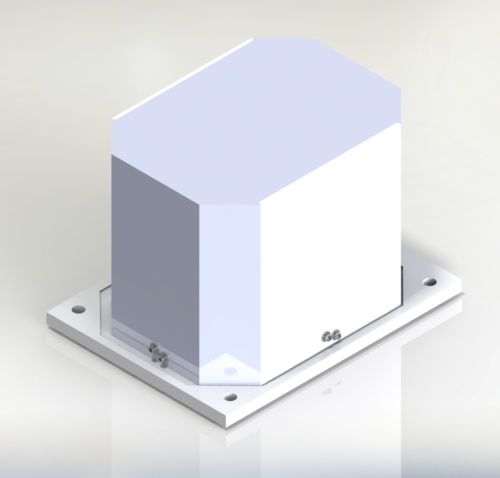
\includegraphics[width=0.5\textwidth]{figures/payload_render.pdf}
%		\caption{Payload Final Design}
%		\label{fig:payload_render}
%	\end{center}
%\end{figure}
%%
%\begin{figure}[h!]
%	\begin{center}
%		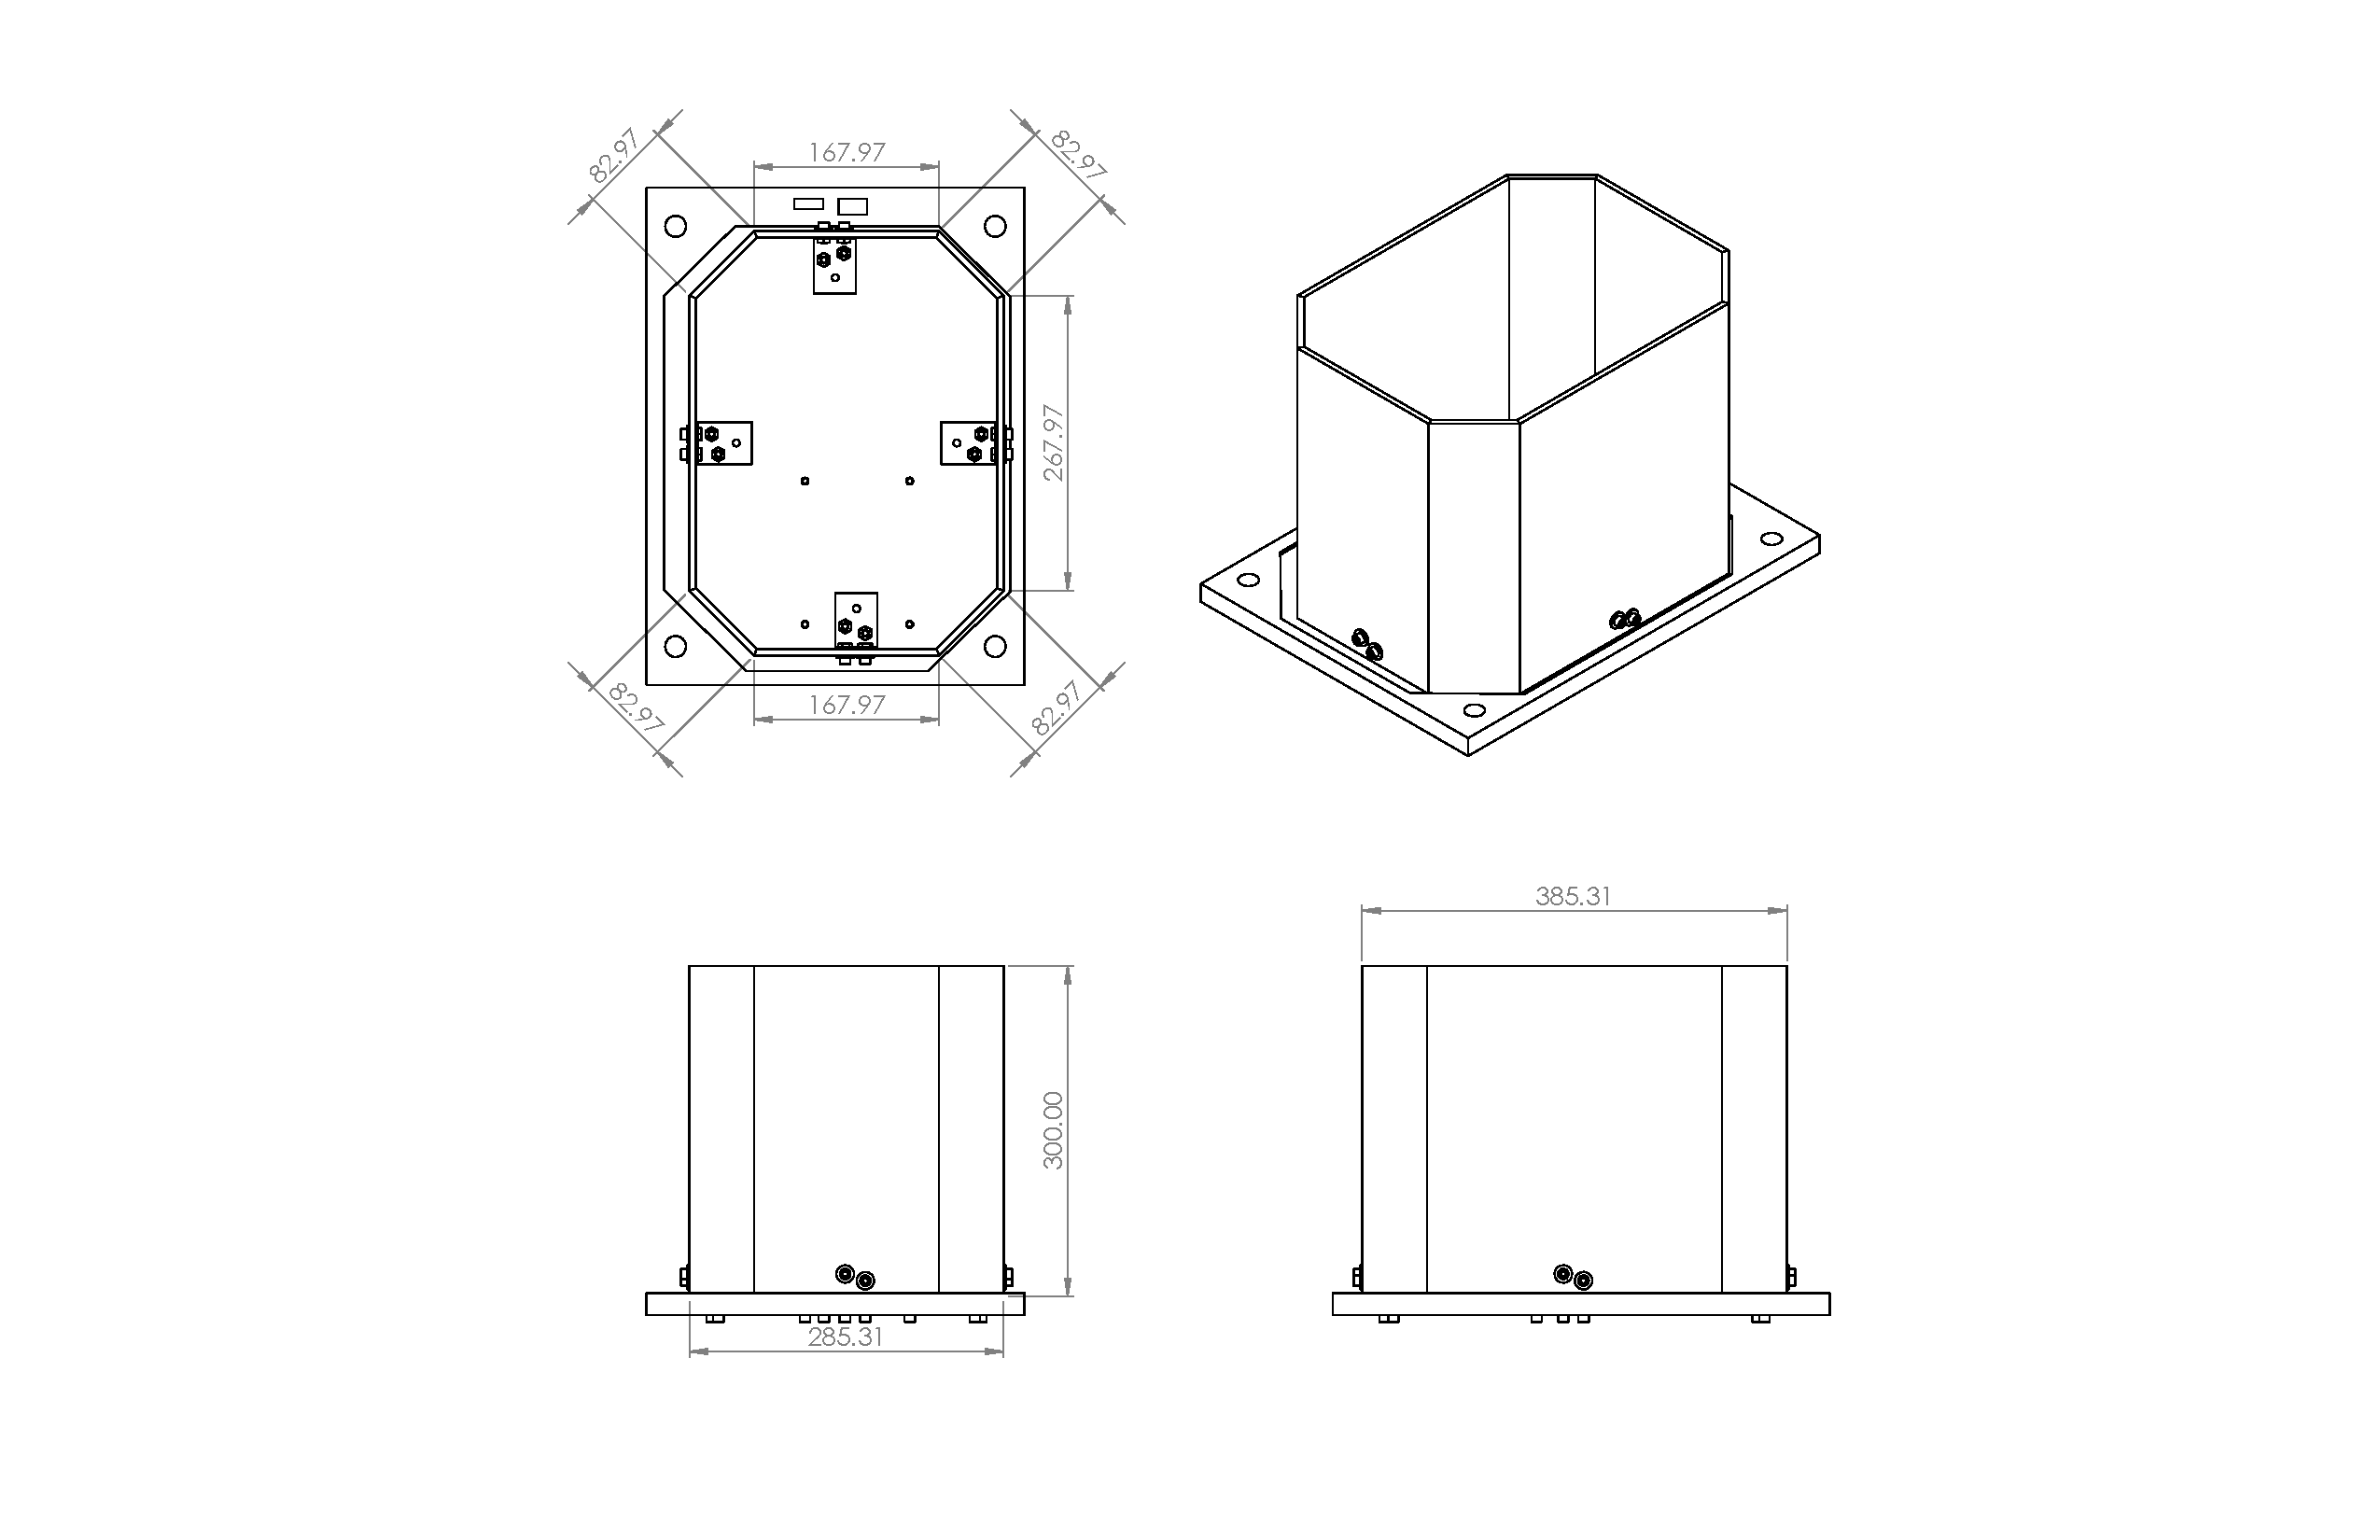
\includegraphics[width=100 mm, scale=1]{figures/payload_dimensions.PDF}
%		\caption{Payload Dimensions}
%		\label{fig:payload_dim}
%	\end{center}
%\end{figure}
%
%\begin{figure}[h!]
%	\begin{center}
%		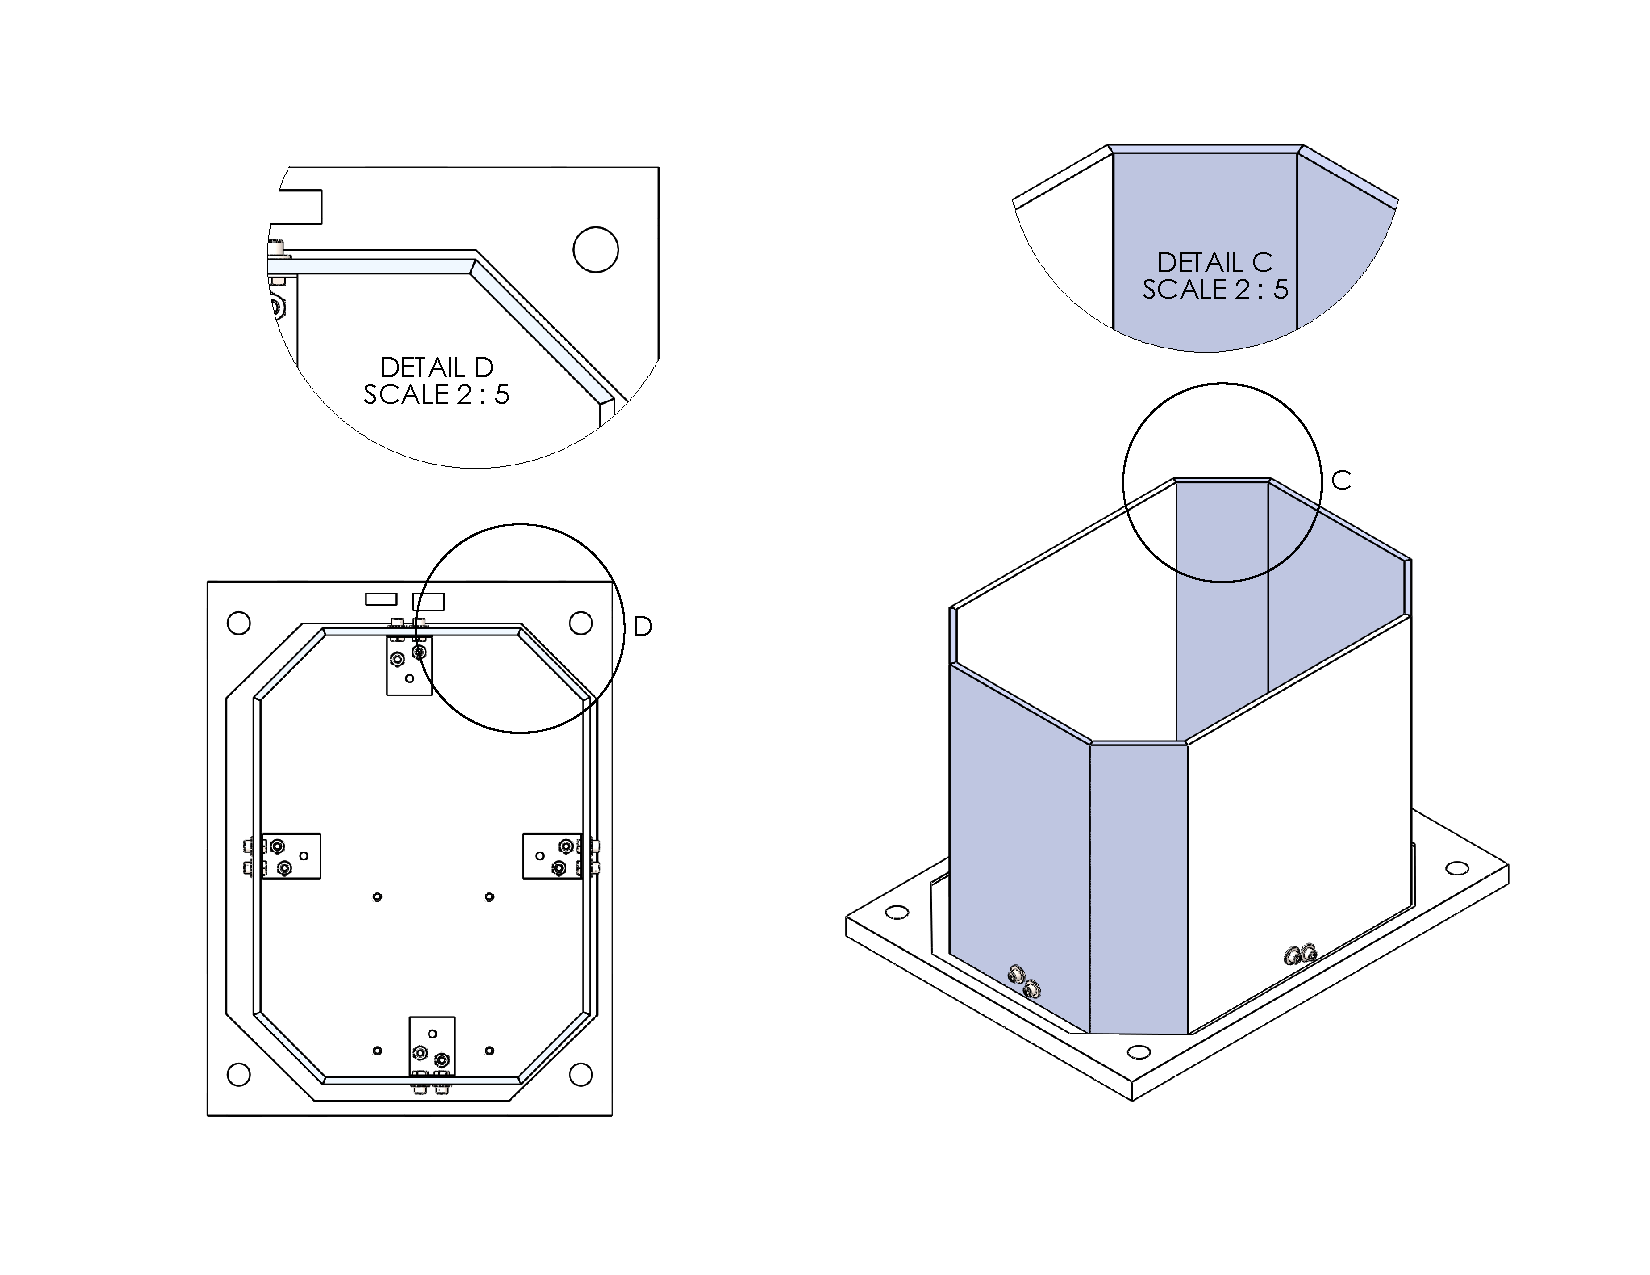
\includegraphics[width=100 mm, scale=1]{figures/payload_corners.PDF}
%		\caption{Payload Corners}
%		\label{fig:payload_corn}
%	\end{center}
%\end{figure}
%%%%%call out a figure.       ~\ref{fig:}
%Subsections:
%Talk about general design of each component or payload part.  Go into detail about choice of materials, placement, and reasoning for the success of the mission.  Also, try to include either real photos, CAD designs or any other relevant graphic.  
%\subsection{MiniPIX}
%MiniPIX
%\subsection{Flight Computer and Sensors}
%Flight Computer and Sensors (include the electric schematics)
%\subsection{Astrobiology}
%Astrobiology (lots of CAD designs)
%\subsection{Payload Structure and Outer Shell}
%Outer Shell (CAD designs and choice of materials)
%Notes:
%Outer material is Kydex from McMasterCarr
%Part PVC and part acrylic
%Manufacturer Specs:
%	https://www.mcmaster.com/acrylic/pvc
%	hydrophobic
%	UV resistant - no sun deterioration
%	3/16 inch thick
%	Color - white
%	Temperature range from -40 F to 150 F
%	Tensile Strength of 6,100 psi
%	Impact strength 15.00 ft.-lbs./in 
%	UL 94V0
%Commonly used for vehicle interiors and equipment housings, this material maintains its shape after heating and forming. It is also known as Kydex. These sheets resist corrosive chemicals and cleaning solutions. One side is smooth; the other side is coarse to mask scratches, scuffs, and fingerprints.
%
%Coated iron bolts, standard size for heavy mounting options
%Nickle plated L-brackets and brackets for wall mounting
%Machine cut to specifications (will include a figure here with all the dimensions)
%\begin{figure}[h!]
%	\begin{center}
%		\includegraphics[width=\textwidth]{figures/[figure name here]}
%		\caption{Payload Final Design}
%		\label{fig:payload_design}
%	\end{center}
%\end{figure}
%
%\begin{figure}[h!]
%	\begin{center}
%		\includegraphics[width=\textwidth]{figures/[figure name here]}
%		\caption{Picture of payload mounted onto gondola}
%		\label{fig:payload_gondola}
%	\end{center}
%\end{figure}
